\documentclass[12pt,oneside]{fithesis2}


\usepackage[english]{babel}
\usepackage[utf8]{inputenc}
\usepackage{lmodern}
\usepackage[T1]{fontenc}
\usepackage{csquotes}

\usepackage[scaled=0.86]{berasans}
\usepackage[scaled=1.03]{inconsolata}

\usepackage{xcolor}
\definecolor{dark-red}{rgb}{0.6,0.15,0.15}
\definecolor{dark-green}{rgb}{0.15,0.4,0.15}
\definecolor{medium-blue}{rgb}{0,0,0.5}

\usepackage[plainpages=false, pdfpagelabels, unicode]{hyperref}

\usepackage{enumitem}
\usepackage[final]{microtype}
\usepackage[top=3.5cm, bottom=4cm, left=3cm, right=3cm]{geometry}	% pc version
%\usepackage[top=3.5cm, bottom=4cm, left=3.5cm, right=2.5cm]{geometry}	% print version

\usepackage[backend=biber,style=ieee]{biblatex}
\addbibresource{thesis.bib}

\usepackage{minted}
\setminted{frame=single, fontsize=\footnotesize}

\usepackage{multicol}
\usepackage{subcaption} 

\usepackage{tikz}
\usetikzlibrary{trees, calc, shapes.arrows, shapes.geometric, shapes.multipart}

\widowpenalty10000
\clubpenalty10000



\thesislang{en}
\thesistitle{GPU-based speedup of EACirc project}
\thesissubtitle{Bachelor Thesis}
\thesisstudent{Jiří Novotný}
\thesiswoman{false}
\thesisfaculty{fi}
\thesisyear{Spring 2015}
\thesisadvisor{RNDr. Petr Švenda, Ph.D.}



\newcommand{\todo}{
	\noindent
	{\large\color{red}\textbf{TODO}}
}

\begin{document}
\FrontMatter
	\ThesisTitlePage
	\begin{ThesisDeclaration}
		\DeclarationText
		\AdvisorName
	\end{ThesisDeclaration}
	\begin{ThesisThanks}
		I thank CRoCS laboratory for provision of workspace and hardware resources to make this thesis happen. I would like to thank Petr Švenda for leading my work and Martin Ukrop for endurance to answering my numerous question about EACirc insides.
		
		\bigskip
		
		\noindent
		Last but not least, I would like to thank my family for continuous support and for help with language aspects of my bachelor thesis.
	\end{ThesisThanks}
	\begin{ThesisAbstract}
		The main focus of this thesis is to bring support for GPU acceleration into EACirc project in order to speed-up the most computationally demanding part. The chosen part is implemented using GPGPU and the achieved speed-up is measured. The thesis also elaborates in build task automation and refactoring of the basic project structure.
	\end{ThesisAbstract}
	\begin{ThesisKeyWords}
		acceleration, CUDA programming, optimization, build configuration, GPU, GPGPU, EACirc, software circuit, randomness testing
	\end{ThesisKeyWords}
	\tableofcontents

\MainMatter
\chapter{Introduction}
Random data and the concept of randomness are used in many branches of informatics. However, one of the fundamental ways how to use these principles is in cryptography and IT security. For instance, let there be a communication among several entities. The main content of the communication is meant to stay hidden from other entities, thus the communication needs to be encrypted by a chosen encryption protocol. The potential attacker\footnote{The one who wants to know the hidden content of the encrypted communication without permission of legal participants.} could intercept some encrypted messages and subject them to analysis. On the basis of certain traits of the protocol or similarities among the individual messages the encryption could be broken and the hidden content of the communication could be read by the attacker. Therefore, the goal of encryption protocols is that the encrypted messages are not similar or do not have some characteristic traits. In other words, the encrypted messages must look like random data to the attacker. However, this is very difficult to be ensured.

That is why tools have been created to test randomness, and thus quality, of ciphers. One of these tools is called EACirc and is being developed at the Faculty of Informatics of Masaryk University in CRoCS laboratory (Centre for Research on Cryptography and Security). It can tell how much the input data are close to the referential random data.\footnote{This is only an approximative explanation. The exact definition and meaning of EACirc results are described in Martin Ukrop's thesis Usage of evolvable circuit for statistical testing of randomness~\cite{ukrop_thesis} since the accurate understanding of EACirc tool is not relevant for this thesis.} To achieve this EACirc uses raw computation power. However, the computations are not run in parallel. If it was the case the whole process would be significantly speeded-up. Faster evaluation could advance capabilities of EACirc and help to test the randomness in a more detailed manner. Speeding-up the EACirc is the primary objective of this thesis.

The speed-up of EACirc is achieved with running some chosen computations on a GPU. The GPU must have got a build-in support of a general purpose programming (GPGPU). Such chip can perform not only algorithms used in rendering of computer graphics but also almost every other algorithm that is runnable on a CPU. The main difference in comparison with CPU is that the CPU is optimized to minimize latency whereas GPU is optimized to maximize throughput. Latency is the time needed to start and finish the execution of a single instruction including time to load necessary data. On the other hand, throughput\label{throughput} is a number which means how many instructions can be processed per one time unit.~\cite{professional_cuda} Since some parts of EACirc process a lot of data with algorithms which does not need to be optimized for latency\footnote{An algorithm that needs to be optimized for latency in order to maximize performance is that one which has lots of edges in it's control flow graph.} the use of GPU's is suitable.

Several different solutions exist on the market which can be used for GPGPU programming. Each solution provides different special features. The solution used for this thesis is called CUDA~\cite{about_cuda} and it is a proprietary technology developed by NVIDIA.~\cite{nvidia} The decision to use CUDA was taken by my advisor.

Since the performance of GPGPU is dependable on the used hardware the achieved speed-up was measured by an experimental method. The benchmarks took place particularly on machines which are being used at CRoCS laboratory for their own computations and are capable to run CUDA programs.

\bigskip

To set EACirc project for using CUDA, a non-trivial intervention into the settings of the project was needed. If the original settings of EACirc had been applied then this intervention would have resulted into a chaotic and further unmaintainable project. Therefore, in addition to the primary objective of this thesis to speed-up EACirc, the secondary objective is to remade the settings completely from scratch in order to prevent the problems that emerged by using CUDA. For this purpose an open-source tool CMake~\cite{cmake} was used that was developed by Kitware corporation~\cite{kitware}.

\bigskip

The text of this thesis was typeset in \LaTeX{} using \textit{fithesis2} package created by Stanislav Filipčík~\cite{fithesis}. The codes fragments which appears in text are typeset using \LaTeX{} package \textit{minted}~\cite{minted} in version 2.0.





\chapter{CUDA}
As stated on the NVIDIA website \cite{about_cuda}, "CUDA is a parallel computing platform and programming model that enables dramatic increases in computing performance by harnessing the power of the graphics processing unit (GPU)." The strengths and weaknesses of GPU lie in it's architecture and in differences from CPU. A GPU that is able to execute CUDA programs is addressed as \emph{CUDA capable device} or simply as the \emph{device}.

\begin{figure}[H]
	\centering
	\includegraphics{figures/gpu-devotes-more-transistors-to-data-processing.png}
	\caption{"The GPU Devotes More Transistors to Data Processing." NVIDA. \cite{cuda_guide}}
	\label{fig:cpu_vs_gpu_arch}
\end{figure}

The figure~\ref{fig:cpu_vs_gpu_arch} shows a high level view of the CPU and GPU architecture. They both contain the same parts: DRAM, Cache, Control, and ALU. DRAM and Cache are memory units, the difference is that Cache is much smaller but significantly faster. The Control unit is responsible mainly for instruction fetching, decoding, etc. ALU is simply a worker that processes the input data. CPU's Control unit and Cache is much bigger and focuses on flow control and data caching in order to reduce the latency. The GPU's counterparts are simpler but multiplied, which allows to focus on data processing (throughput) and data parallelism. It is worth mentioning that the DRAM of a GPU is significantly faster in order to supply enough data to the big number of ALUs and to keep them busy.\footnote{The memory model of GPU is described in section~\ref{memory_hiearchy}.}

The performance of GPU is mainly measured by two variables: throughput and memory bandwidth. Since GPU is mainly used to compute with real numbers throughput\footnote{For definition of throughput see section~\ref{throughput}.} is expressed in units of floating-point operations per second (FLOPS)\footnote{Floating-point operation is an operation on floating-point numbers which in informatics represents real numbers according to the international standard IEEE 754.}. Memory bandwidth is the amount of data that can be processed per unit of time which is expressed in units of bytes per second (Bps).~\cite{professional_cuda} The figures~\ref{fig:gpu_throughput} and~\ref{fig:gpu_bandwith} show the theoretical maximum performance achievable on NVIDIA GPU's in contrast to Intel CPU's in terms of throughput and bandwidth.

\begin{figure}[H]
	\centering
	\includegraphics[width=0.7\textwidth]{figures/floating-point-operations-per-second.png}
	\caption{GPU vs CPU theoretical throughput. "Floating-Point Operations per Second for the CPU and GPU," NVIDIA.~\cite{cuda_guide}}
	\label{fig:gpu_throughput}
\end{figure}

\begin{figure}[H]
	\centering
	\includegraphics[width=0.7\textwidth]{figures/memory-bandwidth.png}
	\caption{GPU vs CPU theoretical bandwidth. "Memory Bandwidth for the CPU and GPU." NVIDIA.~\cite{cuda_guide}}
	\label{fig:gpu_bandwith}
\end{figure}

\section{Hardware architecture}
\label{cuda_architecture}

In both, CPUs and GPUs, DRAM (figure \ref{fig:cpu_vs_gpu_arch}) is significantly slower than ALU. If an ALU requires some data from DRAM, the ALU must wait hundreds of clock cycles for the data to became available (see latency). The waiting is highly ineffective and it is usually solved with some technique for latency-hiding. One of these techniques is executing another thread's instruction which has its data available. The difference between CPU and GPU is how often happens that an instruction wants data from DRAM.

Current CPUs use SIMD (Single Instruction, Multiple Data) execution model.~\cite{professional_cuda} It processes a vector of data with only one instruction. The data in CPU are cached massively to reduce latency\footnote{Data caching is a technique to avoid waiting for data which are stored in a slow storage by introducing memory hierarchy. When data are requested they are firstly searched for in faster memory. When they are not found (cache miss) then a slower memory is searched as long as they are found. Then they are promoted to the faster memory to become available to subsequent requests (cache hit). The data stored in cache which were not accessed for a long time are replaced with a new ones.} and so the ALU does not need to wait. Thus, if big data are not accessed in a wrong way the probability of cache miss is low and switching context to a different thread can be relatively expensive operation.

The execution model of CUDA is called SIMT (Single Instruction, Multiple Threads).~\cite{professional_cuda} Instead of vector of data, a \emph{vector of threads} is executed with one instruction simultaneously. The vector of threads resides in one of the control units. Each thread of the execution vector is then mapped to an ALU related to the control unit. Each control unit has it's own cache. Since the cache is smaller, the cache miss is going to happen more often and another vector of threads, which has all its resources available, is executed. The switching of a thread context is done instantly with null overhead.\footnote{The section~\ref{memory_hiearchy} describes how is this achieved.} Therefore, to keep the GPU busy, more threads than the number of ALUs must be running.

In CUDA terminology the control units are called \emph{Streaming Multiprocessors} (SMs). Each SM has its own ALUs referred to as \emph{cores}. The single thread vector is composed of 32 threads and this is called \emph{warp}. The SIMT architecture implies that all threads of the warp are performing the same instruction simultaneously at the same time.~\cite{cuda_guide}


\section{Thread hierarchy}
\label{thread_hierarchy}

The SIMT architecture of GPU is well suited and designed for computational problems that can be optimized using data parallelism.~\cite{professional_cuda} Data parallelism is a parallelization technique that divides the input data to the independent parts and executes them separately (but evenly) on parallel computing nodes. The final result is then composed from each sub-result.~\cite{data_parallel_algorithms} CUDA platform supports this technique through kernels and thread hierarchy.

In CUDA context a \emph{kernel} is a top-level function that is runnable on CUDA capable devices.~\cite{cuda_guide} It is recommended that the kernel processes only the smallest portion of input data that can be processed separately.~\cite{data_parallel_algorithms} For instance, when adding two vectors the kernel should just add two corresponding scalars of the vector.

For each kernel that is running a separate lightweight thread is created on the device. As shown in figure \ref{fig:grid} a group of threads is forming a \emph{block} and a group of blocks is forming a \emph{grid}. Each thread has got unique ID dependant on its position in the block and each block has unique ID dependant on its position in the grid\footnote{The grid might have up to 3 dimensions.~\cite{cuda_guide}}.

\begin{figure}[H]
	\centering
	\includegraphics[scale=0.9]{figures/grid-of-thread-blocks.png}
	\caption{"Grid of Thread Blocks." NVIDIA. \cite{cuda_guide}}
	\label{fig:grid}
\end{figure}

The dimensions of the grid should correspond to the dimensions of the computational problem. In the example of adding vectors the grid should have the same width as the number of scalars in the vector. Since each thread has a unique ID the kernel knows which scalars to add and where to put the result into the final vector.

The execution of a single kernel is initiated as soon as the device has enough available resources to run a whole block.\footnote{Threads of the same block are running concurrently.}~\cite{cuda_guide} This constraint allows that the threads of one block can communicate with each other (see section \ref{memory_hiearchy}) and that the computational problem can be scaled across different types of CUDA GPUs that disposes with other hardware capabilities\footnote{For instance the number of cores or available memory.}.\footnote{Any program scales if and only if a similar performance is achieved for arbitrary size of input data or across different hardware.~\cite{cuda_best_practices} It is recommended that any well optimized program for CUDA scales.} The execution order of the blocks is not defined.

To fully utilize the device the size of the block should be multiple of a warp size\footnote{For current devices the warp size is 32 (see. section~\ref{cuda_architecture}).}. Each block is mapped to a single SM\footnote{For definition of Streaming multiprocessor (SM) see~\ref{cuda_architecture}.}. On a single SM several blocks may be active but the exact number is dependant on the GPU hardware parameters. Depending of the number of SMs several block may be run in parallel. This is fully done automatically by the CUDA platform. However, the programmer should know these constraints to produce optimized code for each device.\footnote{For various optimization techniques for CUDA platform see~\cite{cuda_best_practices}.}

\section{Memory hierarchy}
\label{memory_hiearchy}

CUDA devices dispose with a multi level memory model. Each level differs in size, speed, and accessibility. The main levels are \emph{global memory}, \emph{shared memory}, and \emph{local memory}.\footnote{In heterogeneous programming the GPU global memory is denoted as subset of \emph{device memory} and CPU memory is denoted as \emph{host memory}. More about heterogeneous programming is in section~\ref{heterogeneous_programming}.}~\cite{cuda_guide}

The global memory is the slowest and the biggest. The data living in the global memory are accessible everywhere in the device. The access to the data is done via 32-, 64-, or 128-byte transactions. The access should fulfil several constraints to achieve maximum performance. One of these restrictions is a coalesced access.\footnote{Other constraints are not relevant for this thesis.} The coalesced access appears if every thread in the block order reads or writes on the subsequent address simultaneously. The global memory should be mainly used for kernel's input/output data and the number of accesses should be minimal.

The shared memory is fast. It is almost as fast as registers and hundreds of times faster than the global memory. It resides in Streaming Multiprocessor's (SM) cache. The data are accessible only by threads of the same block. The number of running blocks on SM is mainly determined by the size of the shared memory required for a single block, which should be known before the block starts executing. Again, there are access restriction for maximum performance. The address space of the memory is alternately divided into 32 (warp size) memory banks of size 32- or 64-bytes. Each thread of the warp should access the different memory bank, which will result in only one transaction. Otherwise the access would be serialized to the number of transactions depending on the maximum number of accesses to one memory bank.\footnote{If multiple threads are requesting value from one address the access will not be serialized but the value will be broadcast resulting only in one transaction.}

The performance of the local memory is almost the same as of the global memory which is slow. The data lives only for the lifespan of a thread and is accessible only by the owning thread. The local memory is only used in a few scenarios described in CUDA C Programming guide~\cite{cuda_guide} in section Device Memory Accesses.

Besides global, shared and local levels of memory a \emph{constant memory} exists.\footnote{There is also a \emph{texture memory} but its description is irrelevant for this thesis. For more informations see~\cite{cuda_guide}}~\cite{cuda_guide} It is a special kind of memory that is meant for constants and is implemented in almost the same way as the global memory. A single access to the constant memory is as slow as an access to the global memory. Since the data in this memory are constants (read-only values) they can be massively cached and the subsequent readings are as fast as readings from shared memory. Lifespan of the data living in the constant memory is the same as of the data living in the global memory.

Every other suitable variable of the scope of a kernel is placed into register. Registers are very fast. The number of registers for each Streaming Multiprocessor~(SM) is large so that each SM may have a lot of active threads and to switch their context easily.\footnote{See SIMT architecture and switching of thread context in section~\ref{cuda_architecture}.} The number of active blocks and threads is determined by the count of used registers by one kernel.

\section{Heterogeneous programming}
\label{heterogeneous_programming}

A heterogeneous system is a system composed of more than one kind of processor.~\cite{professional_cuda} The CUDA philosophy supposes that CUDA executes on a physically separate \emph{device} (GPU) that acts as a coprocessor to the program that is running on the \emph{host} (CPU). The state of the device and the host is stored in their own physically separate memory space referred to as the \emph{device memory} and the \emph{host memory}. Therefore, the host program is in charge of the device resources and manages launching of kernels.~\cite{cuda_guide}

The most often used scenario of kernel launch including device and host resource management is as follows:
\begin{enumerate}[noitemsep]
	\item Host program allocates the space for the input and output data in the host memory.
	\item Host program allocates the space for the input and output data in the device memory.
	\item Host program populates the space for input data in the host memory.
	\item Host program sends the input data to the device.
	\item Host program configures and launches the kernel on the device.
	\item Device program is executed.
	\item Host program copies the final results from the the device to the host.
	\item Host program processes the results. 
\end{enumerate}

\noindent
Since most of these actions are input/output operations, they may be performed either synchronously or asynchronously.\footnote{A synchronous operation blocks execution of the host program for the duration of the operation. An asynchronous operation does not block the execution of the host program and the incoming/outgoing transmission can overlap with computation. The host program is then notified whether the asynchronous operation succeeded or failed.~\cite{async_io}} The execution of the kernel on the device is always asynchronous.~\cite{cuda_guide}

\section{Compute capabilities}

As producing an optimized code for CUDA devices is closely linked to their hardware parameters~\cite{cuda_best_practices} and because with almost every new product line of NVIDIA GPUs new features are introduced, NVIDIA established a system for backward and forward compatibility. The GPUs were divided to the classes reflecting technical parameters and runtime features of CUDA platform. These classes are referred to as compute capabilities.\footnote{For full list of compute capabilities corresponding to the date of release of this thesis see CUDA~C~Programming~Guide \cite{cuda_guide} section G.~Compute~Capabilities}.

\section{Programming language}
\label{cuda_lang}

The main programming languages for CUDA are \emph{C} and \emph{C++} which are enriched by several CUDA specific keywords. Since \emph{C++} is a high-level language, some \emph{C++} features are not supported in the device code. The source code for the device and for the host may be mixed together and placed into one source file jointly.~\cite{cuda_guide}

The listing \ref{listing:cuda_example} shows a sample of CUDA code which produces a sum of two vectors on the device. The sample follows the scenario of launching the kernel as described in section \ref{heterogeneous_programming}.

However, one caution should be remembered before porting an algorithm to the CUDA platform. If an algorithm contains an \emph{if-then-else} statement and any thread of the warp evaluates the condition differently then the different execution paths are serialized. The execution paths merge after every thread of the warp finished its execution path. Fortunately some techniques exists to avoid this artefact. This principle also applies on other language control flow constructs such as loops, goto statements, etc.~\cite{cuda_guide}

\begin{listing}[h]
	\begin{minted}[autogobble, linenos, frame=single, xleftmargin=2em]{cuda}
	// kernel definition (the __global__ keyword declares the kernel)
	__global__ void vector_add_kernel( float* a, float* b, float* c )
	{
		// the id of this thread in the block as a local variable
		int i = threadIdx.x;
		
		// add corresponding scalars of the vector and store the result
		// vectors a, b, and c are stored in the global memory
		c[i] = a[i] + b[i];
	}
	
	int main()
	{
		float* host_a, * host_b, * host_c;
		float* device_a, * device_b, * device_c;
	
		// allocate vectors on the host
		cudaMallocHost( &host_a, SIZE * sizeof( float ) );
		cudaMallocHost( &host_b, SIZE * sizeof( float ) );
		cudaMallocHost( &host_c, SIZE * sizeof( float ) );
		
		// allocate vectors on the device
		cudaMalloc( &device_a, SIZE * sizeof( float ) );
		cudaMalloc( &device_b, SIZE * sizeof( float ) );
		cudaMalloc( &device_c, SIZE * sizeof( float ) );
		
		// copy input vectors from host to device
		cudaMemcpy( device_a, host_a, size, cudaMemcpyHostToDevice );
		cudaMemcpy( device_b, host_b, size, cudaMemcpyHostToDevice );
		
		// launch kernel with only 1 block of size SIZE
		// a special CUDA syntax is used
		vector_add_kernel<<< 1, SIZE >>>( device_a, device_b, device_c );
		
		// retrieve the result from device
		// although the launch of the kernel is asynchronous this function 
		// waits untill the execution of the kernel is not finished
		cudaMemcpy( host_c, device_c, SIZE, cudaMemcpyDeviceToHost );
		
		// free memory on the device
		cudaFree( device_a );
		cudaFree( device_b );
		cudaFree( device_c );
		
		// free memory on the host
		cudaFreeHost( host_a );
		cudaFreeHost( host_b );
		cudaFreeHost( host_c );
		
		return 0;
	}
	\end{minted}
	\caption{A sample program of vector addition on CUDA platform.}
	\label{listing:cuda_example}
\end{listing}

\section{Tools}

NVIDIA provides the necessary tools for the development on CUDA platform through CUDA Toolkit package.~\cite{cuda_toolkit} The source files of CUDA programs must be compiled by a special compiler. The compiler that comes with the CUDA Toolkit is called \texttt{nvcc}.~\cite{cuda_compiler} The compiler supports mixing the code for the host with the code for the device. The \texttt{nvcc} identifies the code for the device and compiles it to an intermediate object file. The remaining code for the host is then forwarded to the ordinary compiler for \emph{C/C++} like \texttt{gcc}, \texttt{clang}, or \texttt{cl}. The object files from the \texttt{nvcc} and the host compiler are then linked into the binary form using ordinary linker or by \texttt{nvcc}. Therefore, the formed binary includes both the code for the host and for the device.

Debugging of the device code is slightly different from debugging of the code for the host. It requires a special debugger. The one that comes with CUDA Toolkit is called \texttt{cuda-gdb}.~\cite{cuda_gdb} The interface of this tool is almost the same as the interface of the known Linux compiler \texttt{gdb}.

%The CUDA Toolkit also provides tools for kernel profiling and feature rich libraries for the common computation problems on CUDA platform.





\chapter{CMake}

To set EACirc project for using CUDA, an intervention into the settings of the project was needed. Below the original settings and workflow of EACirc are described. However, this settings had to be remade from scratch.

The EACirc sources consist mainly of \emph{C} and \emph{C++} code. The code is divided into reasonably logical sections, but the overall structure and concept of the project are monolithic\footnote{A monolithic binary is an executable that does not need any other dependencies or resources at a runtime. In other words, the binary is independent.}. This leads to compilation of all sources into one big executable of approximately 9~MB, which takes some non-trivial time.

On top of this EACirc is developed as a cross-platform application. To provide native builds for each supported platform (Windows~\cite{win} and Linux) a special makefile or an IDE specific project file are used simultaneously. They describe how to build the application. When a change in the build is introduced, e.g. a new source file is added, the change has to be manually implemented to all makefiles to provide consistency. This workflow is not easy to maintain as the violation of these rules can cause an uncomfortable pitfall.

To solve these problems the CMake~\cite{cmake} tool was integrated into the project of EACirc along with some changes of the basic structure of EACirc. The CMake tool is developed and maintained by Kitware, Inc.~\cite{kitware} as an open-source software. The main purpose of this tool is to provide native builds of cross-platform applications and to minimize the effort to maintain the project.

Although there are many similar tools as CMake and some of them provide better features they are not so widely supported. For instance, CMake generates project files for almost every common IDE and some of these IDEs come with a built-in support for CMake.

\section{CMake toolset}

The CMake is actually a set of several tools that provide for building, testing, and deploying of user's \emph{C} or \emph{C++} project. These tools can be installed on Linux, Windows, or MacOSX. The CMake toolkit consists of the main tool \texttt{cmake} and the supportive \texttt{ccmake} (or \texttt{cmake-gui}), \texttt{ctest}, and \texttt{cpack}.~\cite{cmake_docs}

The \texttt{cmake} tool takes a configuration file called \texttt{CMakeLists.txt} distributed with the project source files and generates the platform specific makefiles as an output. Then the user invokes a platform specific tool for building -- usually \texttt{make}, \texttt{ninja}~\cite{ninja}, or \texttt{MSBuild}.~\cite{msbuild} If the process is successful the native binaries of the project are now made.

The \texttt{ctest} tool provides a simple platform for project testing. If the build is successful the user can run some custom made tests on the binaries.

The \texttt{cpack} tool provides a cross-platform mean to deploy your application on the target system.

The remaining \texttt{ccmake} and \texttt{cmake-gui} are just more convenient ways to use a \texttt{cmake} tool since \texttt{cmake} has only a command line interface. The former provides a TUI\footnote{Text-based user interface (TUI)} and the latter provides GUI\footnote{Graphical user interface (GUI)}.

\section{A closer look at the \texttt{cmake} executable}

The \texttt{cmake} executable is not just a dummy build-system. The process of generating a makefile is quite sophisticated. First, the user chooses the \emph{source directory} and the \emph{build directory} and then invokes the \texttt{cmake} command in a \emph{build directory} with appropriate parameters. The subsequent process consists of several phases -- selection of a native build-system (in a CMake terminology referenced as a \emph{generator}), configuration based on a user-specific input, and the generation of a makefile itself.\footnote{Note that the exact scheme of this process can differ according to which interface of CMake is used -- i.e. \texttt{cmake}, \texttt{ccmake}, or \texttt{cmake-gui}.}~\cite{cmake_docs}

The \emph{source directory} is simply a directory where the project sources are located as well as the top-level \texttt{CMakeLists.txt} file which is distributed with the sources. The build directory is an empty user-created directory in which the user wants the binaries to be build.

The selection of the \emph{generator} depends on the user's platform, on the user-installed native build-systems, and on the user's intentions. The generator used on Linux is usually \texttt{make} or \texttt{ninja}. If the user wants to generate project files to a specific IDE, appropriate generator can be chosen -- e.g. Visual Studio 2013~\cite{msvc} on Microsoft Windows~\cite{win}. Usually the selection of the appropriate generator is done by CMake automatically.

The subsequent phase is configuration. Here the user specifies variable options for the build that the project supports. For instance, some features of the application can be switched on/off or the location of a third party dependencies can be specified. Also the different build configuration can be switched, i.e. release or debug.

If the configuration is correct then the makefile is successfully created in the \emph{build directory}. Then the user just invokes the appropriate tool to execute the makefile and the binaries are build.

It is worth mentioning that the makefile automatically detects any changes made in the \emph{source directory}. So the user invokes the \texttt{cmake} executable just once to generate the makefile or to change the variable options of the build. The makefile also provides a way to install the application and/or to test it.

The minimal and the most common sequence of commands to build and install a project on Linux using the CMake is shown in listing~\ref{listing:cmake_example}.

\begin{listing}[h]
	\begin{minted}[autogobble]{text}
	mkdir <build_directory>
	cd <build_directory>
	cmake <path_to_source_directory>
	make
	make install
	\end{minted}
	\caption{The minimal CMake workflow.}
	\label{listing:cmake_example}
\end{listing}

Note that the \texttt{make} is chosen as a default generator. In addition, the default project settings and configurations are applied. The binaries are installed to the platform specific location, i.g. on Linux it is \texttt{/usr/share/local}.

\section{Changes made to the EACirc repository structure}

There were several changes made to the EACirc repository structure. The new folder design reflects the logical structure of the EACirc philosophy. The changes are shown in the figure~\ref{fig:repository_changes}.

\begin{figure}[h]
	\centering
	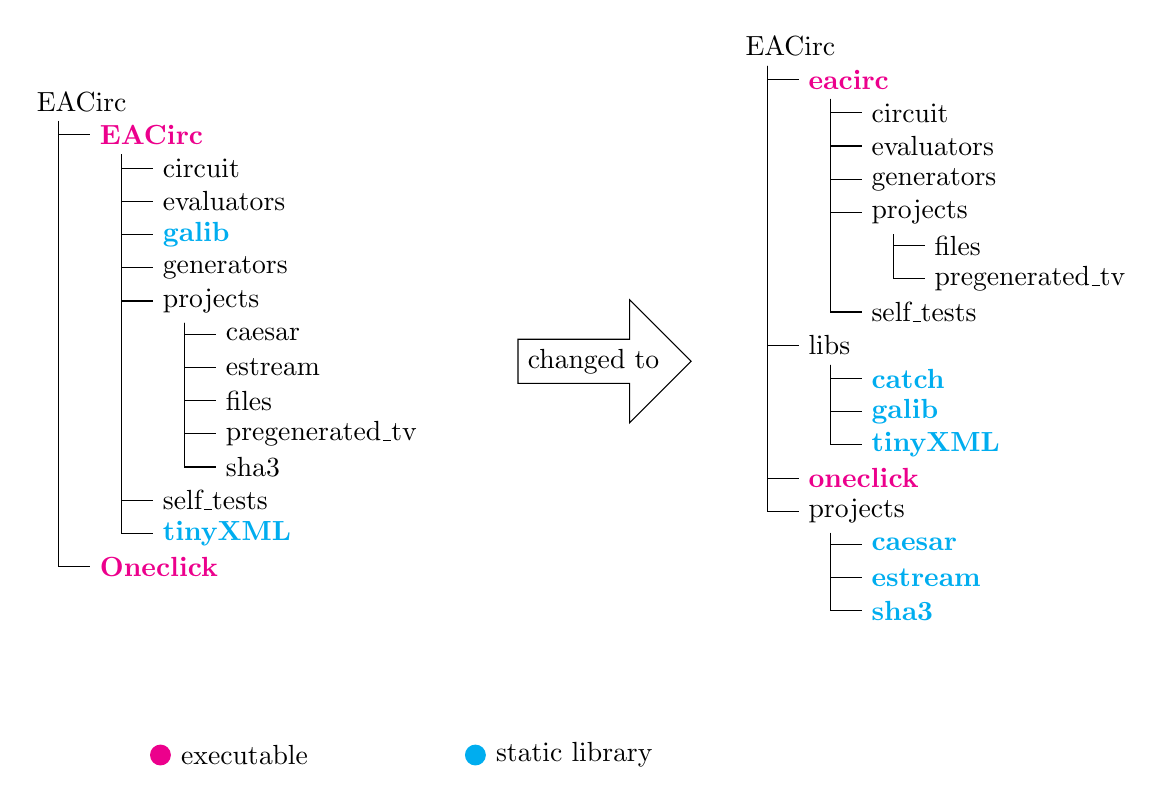
\begin{tikzpicture}[
grow via three points={one child at (0.8,-1.2em) and two children at (0.8,-1.2em) and (0.8,-2.4em)},
edge from parent path={($(\tikzparentnode\tikzparentanchor)+(.4cm,0pt)$) |- (\tikzchildnode\tikzchildanchor)},
growth parent anchor=west,
parent anchor=south west,
every child node/.style={anchor=west}
]
\node at (0,-2em) {EACirc}
	child { node [font=\bf,text=magenta] {EACirc}
		child { node {circuit} }
		child { node {evaluators} }
		child { node [font=\bf,text=cyan] {galib} }
		child { node {generators} }
		child { node {projects}
			child { node {caesar} }
			child { node {estream} }
			child { node {files} }
			child { node {pregenerated\_tv} }
			child { node {sha3} }
		}
		child [missing] {}
		child [missing] {}
		child [missing] {}
		child [missing] {}
		child [missing] {}
		child { node {self\_tests} }
		child { node [font=\bf,text=cyan] {tinyXML} }
	}
	child [missing] {}
	child [missing] {}
	child [missing] {}
	child [missing] {}
	child [missing] {}
	child [missing] {}
	child [missing] {}
	child [missing] {}
	child [missing] {}
	child [missing] {}
	child [missing] {}
	child [missing] {}
	child { node [font=\bf,text=magenta] {Oneclick}
	};
	
\node at (6.5, -4) [single arrow, draw, single arrow head extend=.5cm] {changed to};
		
\node at (9, 0) {EACirc}
	child { node [font=\bf,text=magenta] {eacirc}
		child { node {circuit} }
		child { node {evaluators} }
		child { node {generators} }
		child { node {projects}
			child { node {files} }
			child { node {pregenerated\_tv} }
		}
		child [missing] {}
		child [missing] {}
		child { node {self\_tests} }
	}
	child [missing] {}
	child [missing] {}
	child [missing] {}
	child [missing] {}
	child [missing] {}
	child [missing] {}
	child [missing] {}
	child { node {libs}
		child { node [font=\bf,text=cyan] {catch} }
		child { node [font=\bf,text=cyan] {galib} }
		child { node [font=\bf,text=cyan] {tinyXML} }
	}
	child [missing] {}
	child [missing] {}
	child [missing] {}
	child { node [font=\bf,text=magenta] {oneclick} }
	child { node {projects}
		child { node [font=\bf,text=cyan] {caesar} }
		child { node [font=\bf,text=cyan] {estream} }
		child { node [font=\bf,text=cyan] {sha3} }
	};
	
	\node at (1,-9) [scale=0.8,shape=circle,fill=magenta,label=right:executable] {};
	\node at (5,-9) [scale=0.8,shape=circle,fill=cyan,label=right:static library] {};
\end{tikzpicture}
	\caption{Old vs. new repository structure}
	\label{fig:repository_changes}
\end{figure}

The first and also the smallest change was to name all source folders with only small letters. Next the libraries from 3rd party providers \texttt{catch}, \texttt{galib}, and \texttt{tinyXML} were moved into the separate folder -- the \emph{libs} directory.

Then the so called \emph{projects} were isolated. A \emph{project} in EACirc terminology means a problem solving module. These \emph{projects} are \texttt{caesar}, \texttt{estream}, \texttt{sha3}, \texttt{files} and \texttt{pregenerated\_tv}. Since \texttt{files} and \texttt{pregenerated\_tv} are both just small modules consisting of only one source file, it would be impractical to isolate them. Whereas the big modules \texttt{caesar}, \texttt{estream}, and \texttt{sha3} were moved to the separate folder called the \emph{projects} folder. Each of the isolated projects was remade to compile into a static library.\footnote{There is a plan to remake the projects to modules loaded dynamically at runtime. This would require to compile them separately into the dynamic libraries.}

The content of folders \texttt{eacirc} and \texttt{oneclick} is build into executables which are named accordingly to their corresponding folder. The \emph{projects} which are now compiled into the static libraries are now statically linked to the \texttt{eacirc} executable representing the EACirc tool as a whole. The \texttt{oneclick} executable is a supportive tool for the automated task management developed by Ľubomír Obrátil.~\cite{oneclick}

\section{The new build-system of EACirc}

The new build-system is written on the CMake platform. This platform allows to define custom options for generating the build. A descriptive list of EACirc specific options is given below:

\begin{description}[noitemsep]
	\item[\texttt{BUILD\_ONECLICK}] \hfill \\
	Enable building of Oneclick, the supportive tool for EACirc.
	\item[\texttt{BUILD\_CAESAR}] \hfill \\
	Enable building of the Caesar project.
	\item[\texttt{BUILD\_ESTREAM}] \hfill \\
	Enable building of the Estream project.
	\item[\texttt{BUILD\_SHA3}] \hfill \\
	Enable building of the SHA-3 project.
	\item[\texttt{BUILD\_CUDA}] \hfill \\
	Enable to build the support for CUDA devices. This option is available only if the CUDA Toolkit \cite{cuda_toolkit} is installed on the build machine\footnote{A build machine is a physical or a virtual machine that is used to build the project.} and found by the CMake.
\end{description}

\noindent
Since the \emph{projects} are build into static libraries they must be linked to the \texttt{eacirc} executable at the compile time. This is done automatically when the option for the specific \emph{project} is enabled. In the figure~\ref{fig:deps} dependencies of all the build targets are shown.

\begin{figure}[h]
	\begin{center}
		\includegraphics[width=.8\textwidth]{figures/deps}
	\end{center}
	\caption{EAcirc dependency graph}
	\label{fig:deps}
	\caption*{The static libraries are shown in the rhombus. The executables have a house around them, squares represent interface libraries\footnote{Interface library does not need to be linked against. It consists only of header files.} and the direction of arrows describes dependency of build targets.}
\end{figure}

The build-system is also version aware. The current version is stored in the \texttt{eacirc/Version.h} header file. The version corresponds to git commit hash~\cite{git_book}. This means that for the correct build generation git tools must be properly installed on the build machine and found by CMake.\footnote{If git tools are installed and not found automatically by CMake then the path to git tools can be specified manually.}

The use of CMake and the new options of building EACirc is explained in detail on the Github wiki project page under the Building EACirc section.

\section{Project settings for CUDA}

It is now much easier to set the project for CUDA support with CMake than with ordinal makefiles. When the CUDA Toolkit~\cite{cuda_toolkit} is installed and automatically found by CMake\footnote{If CUDA Toolkit is installed on the build machine but not found by CMake automatically then the path to CUDA Toolkit can be specified manually.} then the option \texttt{BUILD\_CUDA} becomes available. If this option is enabled then the \texttt{eacirc} executable is build by using Nvidia \texttt{nvcc} compiler~\cite{cuda_compiler} and the C~preprocessor macro \texttt{CUDA} is defined causing that the executable will be runnable on CUDA capable devices. When writing a code for CUDA the preprocessor macro \texttt{CUDA} can be queried.





\chapter{Gate Circuit of EACirc}

The purpose of EACirc is to differentiate input data and referential random data from one another without any context. The input data consists of thousands of sample outputs from an arbitrary random generator. These sample outputs are referred to as \emph{input vectors}. The distinction is done by creating a gate circuit which processes the input data and outputs the result. The internal structure of the optimal gate circuit is unknown at the moment of invocation of the EACirc program. However, the optimal form of the circuit is constructed via a genetic algorithm.~\cite{ukrop_thesis}

Genetic algorithms are inspired by processes of reproduction and natural selection in living systems. They search for a satisfactory optimal solution for a given problem. The process of producing the acceptable solution consists of creating a random initial generation of individuals and then iteratively applying evaluation of the generation, selection of the best individuals for the next generation, and creating next generation by applying genetic operators.~\cite{genetic_algorithms}

The functionality of the gate circuit in EACirc is the same as an ordinary digital circuit that is composed from electronic components (\emph{gates}) connected with wires (\emph{connectors}). Each gate is performing some logical function on its input defined by connectors. The whole circuit takes one input vector, which is a fixed amount of logical data, and outputs if the input is random or not.\footnote{Actually the output of a circuit is not only a binary (random/non-random) but contains other information that is further processed.} Since the gate circuit, in the context of EACirc, is stored in the memory of a computer, the implementation differs from the real world.

Producing the final gate circuit via genetic algorithm is an iterative process. In each iteration the whole generation of circuits must be evaluated. The evaluation of a single circuit is done by processing all the input vectors. All of these parts of the process must be done in large quantities to ensure quality, which is a computationally intensive task. Fortunately, the evaluation of a single circuit and even the evaluation of the whole generation can be run effectively in parallel. This thesis focuses mainly on parallelization of evaluation of a single circuit.

The evaluation of a single circuit is suitable for parallelization, particularly for data parallelism on GPGPU and CUDA platform. The size of the input data is relatively small (usually 16~KiB or more)\footnote{The exact parameters of the circuit are runtime variables. The reported values in parenthesis are just the most used but if running on CUDA, bigger values are expected.} The input data are a set of input vectors (usually 1000 vectors). Each input vector is evaluated separately by the same circuit which usually outputs only 1~byte of data. Therefore, the data transfers between host and device via a \emph{slow} PCIe bus will be small.\footnote{The PCIe bus has got a big latency, thus the number of transfers must be minimized or the transfers must be buffered.} The data parallelism can be achieved by mapping of execution of single input data to separate device thread. The single circuit processes different data equally, i.e. the data is different but the execution paths of multiple running circuits are the same.


\section{Software representation of hardware circuit}

The following text describes the CPU implementation and functionality of the gate circuit designed by Martin Ukrop.~\cite{ukrop_thesis} This representation served as a starting point for the GPU implementation.

From informatics point of view, the gate circuit can be described as a directed acyclic graph (DAG) with some other restrictions described further. Each node represents a logical function (\emph{gate}), the edges (\emph{connectors}) of the vertices represents inputs for the individual logical functions and the flow of data. The graph is divided into several layers. Every node in each layer is connected only to nodes which belong to the previous layer. For a graphical presentation of the circuit see figure~\ref{fig:gate_circuit}.~\cite{eacirc_circuit}

\begin{figure}[h]
	\centering
	\includegraphics[width=0.8\textwidth]{figures/gate_circuit.pdf}
	\caption{The dimensions of the gate circuit}
	\caption*{The gates are in blue, the connectors are the black lines. The yellow, green, and red nodes show mapping of data to the gates. The flow of the data is from top to bottom.}
	\label{fig:gate_circuit}
\end{figure}

\subsection{Use memory feature}

The gate circuit has a special feature of using a memory. It allows to process larger input vectors than the maximal width of the circuit input (see figure~\ref{fig:gate_circuit} and \texttt{size\_of\_input}). The input vector is divided into several parts of size \texttt{size\_of\_input} and each part is processed sequentially. A part of output (\texttt{size\_of\_memory}) from current run of the circuit is transfused to the input of the next run (see figure~\ref{fig:gate_circuit} and the yellow nodes). If this feature is not used then the \texttt{size\_of\_memory} is equal to~$0$. Unfortunately, the feature of using a memory was newer used in production. Therefore, the feature is not implemented in GPU version of the circuit.

\subsection{Circuit dimensions}

The circuit dimensions (see figure~\ref{fig:gate_circuit}) are loaded at the EACirc invocation from settings and fixed for the whole runtime of the program. The circuit has got \texttt{num\_of\_layers} layers. All layers except the last one have \texttt{size\_of\_layer} nodes. The last layer has \texttt{size\_of\_output\_layer} nodes. Each node is limited by the same maximum number of allowed connectors.


\section{CPU implementation}
\label{cpu_implementation}

The understanding of CPU implementation of the circuit by Martin Ukrop~\cite{ukrop_thesis} is necessary in order to provide a bridge interface to the GPU implementation and to preserve functionality.

In computer memory the gate circuit is represented as an 1-dimensional array of 32-bit unsigned integers. Each integer has its own meaning. The array is alternately divided into connection layers and function layers as shown in the figure~\ref{fig:circuit_cpu_array}. Each layer is aligned to a multiple of \texttt{genome\_width}.

\begin{figure}[h]
	\centering
	\includegraphics[width=\textwidth]{figures/cpu_genome.pdf}
	\caption{The representation of gate circuit in CPU memory.}
	\label{fig:circuit_cpu_array}
\end{figure}

\subsection{Connector layers}

The connection layers contain connector masks which are represented as 32-bit unsigned integers. Each node has assigned its own connector mask. If the $i$-th bit of the connector mask is \texttt{true} then connection exists from the $n$-th node of the previous layer to the node the connector is assigned to, where $n$ depends on the connector type. There are two types of connectors which are convertible to one another. The types are \emph{absolute connectors} and \emph{relative connectors}.

Relative connector is a representation of a connection which is defined through relative positioning to the node it belongs to. This representation is used in genetic algorithm when creating new generation, i.e. if the circuit is cut in half and crossed with another individual\footnote{Crossing of individuals is one of the types of genetic operators used for creating a new generation of individuals.} the connector remains still valid.

Absolute connector is a representation of a connection by absolute positioning. This positioning is used when the circuit is being executed because then the process of resolving the absolute connector is much faster then resolving the relative connector.

\subsection{Function layers}

The function layers contain function masks which are represented as 32-bit unsigned integers. To each node a special function mask is assigned. The mask contains information about the function type and arguments. For the list of possible function types see EACirc wiki section Gate circuits.~\cite{eacirc_circuit}

\subsection{Circuit interpreter}

The circuit interpreter is responsible for executing the circuit. The interpreter processes each layer of the circuit sequentially. The CPU version uses the dynamic allocation of memory for the inputs and outputs of the currently processed layer. Each invocation of the CPU circuit interpreter on the same circuit (the same circuit is invoked thousand times and more) converts the relative connectors to the absolute connectors. This is a major performance drawback and it could be done only once for each circuit to speed the execution.


\section{GPU implementation}

The GPU implementation source files of the gate circuit is placed in the directory \texttt{eacirc/circuit/gpu\_gate}. The sources are written mainly in \emph{CUDA~C++}\footnote{For the description of \emph{CUDA~C++} language see section~\ref{cuda_lang}} or \emph{C++} programming language using the standard \emph{C++11}.~\cite{std_c++11, cuda_guide} The GPU implementation provides the proper interface for communication with the rest of the program. The GPU circuit representation and the interpreter are written using \emph{C++} templates~\cite{std_c++11} in order to provide multiple sizes of connector and function masks and thus larger circuits.

The GPU implementation is written with the idea of running the code on GPU and on CPU, too. The GPU support is the primary one. Running the code on CPU should by possible after a minimal intervention into the EACirc source codes.\footnote{Running the code on CPU has not been tested yet, but should be possible.} The reason to make the new implementation capable running on GPU and CPU is to maintain only one implementation that is runnable on every machine and provides GPU acceleration if the machine hardware supports it.

\subsection{Circuit representation}
\label{gpu_curcuit_repr}

The GPU implementation cannot use the storage layout of the circuit as the CPU version described in section~\ref{cpu_implementation}, because of the CUDA memory restriction for faster data access.

The circuit is stored as 1-dimensional array of instances of \emph{C++} template class \texttt{gate\_circuit::node} in a \emph{constant memory} of the device. The nodes are stored similarly as layers in CPU implementation using alignment (see figure~\ref{fig:gpu_genome}).

\begin{figure}[h]
	\centering
	\includegraphics[width=\textwidth]{figures/gpu_genome.pdf}
	\caption{The gate circuit stored in GPU constant memory}
	\label{fig:gpu_genome}
\end{figure}


The \texttt{node} class represents circuit nodes that have its own function and connector masks. The reasons of this data layout are to use coalesced memory access for faster data transfers and to better use the caching capabilities of GPU.\footnote{For coalesced access and caching see section~\ref{memory_hiearchy}.} The whole node always resides in one cache line and therefore, only one transaction to load data from constant memory is used. The listing~\ref{listing:gpu_node} shows the basic structure of the node using \emph{C++} code.

\begin{listing}[h]
	\begin{minted}[autogobble, linenos, frame=single, xleftmargin=2em]{cpp}
	template <typename T>
	class gate_circuit {
	public:
		using value_type = T;
		
		class node {
			value_type _func_mask;
			value_type _conn_mask;
		};	
	};
	\end{minted}
	\caption{The GPU representation of circuit node}
	\label{listing:gpu_node}
\end{listing}

\subsection{Converting between CPU and GPU representation}

The template class \texttt{gate\_helper} is responsible for conversion between CPU and GPU representation of the circuit. The conversion is performed on CPU before the circuit definition is sent to device and executed. The gate helper also transfers the relative connectors to absolute connectors, because the GPU interpreter works only with absolute connectors.

\subsection{Interpreter}

The GPU circuit interpreter is contained in template class \texttt{gate\_interpreter}. This class is capable of executing the circuit on GPU and CPU. The reason why this class is written as a template is to support different types of circuits (see~\ref{gpu_curcuit_repr}). One invocation of the circuit interpreter processes only one input vector.

The GPU interpreter processes the data similarly as the CPU version -- one circuit layer after another. The state of the execution is maintained per instance and thus multiple instances must be created for concurrent execution. The inputs and outputs from the currently processed layer are stored in a memory that is allocated outside the class scope. Therefore, different storage spaces may be used when running the interpreter on CPU or GPU. The input and output vectors are passed through a pointer for each circuit execution.

\subsection{Kernel}

The kernel function\footnote{For definition of kernel see section~\ref{thread_hierarchy}.} accepts the following necessary parameters to run the circuit on GPU: pointer to the storage of circuit inputs and outputs, the circuit definition, and the size of the device's shared memory bank\footnote{For the description of the shared memory bank see section~\ref{memory_hiearchy}.}. The listing~\ref{listing:kernel} shows the code.

The kernel computes its ID and the exact position of input and output vectors which are located in the global memory and which the kernel is supposed to process. Then the kernel allocates the space for interpreter layers in a shared memory for the fastest data access. The reason to use shared memory over registers is that the size of shared memory may be specified at the runtime during kernel launch. On the contrary, the size of registers must be known at the compile time. Since the size of the circuit layer is not know at the compile time, the shared memory is used for inputs and outputs of the currently processed layer.

The allocation is done by the CUDA platform automatically when the execution of the block starts. Since the shared memory belongs to the whole block of threads, each kernel must ensure a space for its own execution layers. However, each thread of the warp accesses the data in the shared memory at different addresses simultaneously and the bank conflict\footnote{For the description of bank conflict see~\ref{memory_hiearchy}.} can emerge. The bank conflicts are prevented using a technique called striding. The technique is based on allocation of an extra space for each thread. The size of the extra space is equal to the bank size and is never accessed by any thread, thus each thread of the warp accesses a different bank every time.

\begin{listing}[h]
	\begin{minted}[autogobble, linenos, frame=single, xleftmargin=2em]{cuda}	
	template <class T>
	__global__ void kernel(const byte* ins, byte* outs,
	                       const gate_circuit<T> circuit,
	                       const size_t bank_size)
	{
		const int id = blockIdx.x * blockDim.x + threadIdx.x;
		
		const byte* in = ins + (id * circuit.in_size);
		byte* out = outs + (id * circuit.out_size);
		
		
		extern __shared__ byte memory[];
		
		byte* layers =
		         memory + ((2 * circuit.in_size + bank_size) * threadIdx.x);
		
		gate_interpreter<T> interpreter(layers, &circuit);
		interpreter.execute(in, out);
	}
	\end{minted}
	\caption{The interpreter kernel}
	\label{listing:kernel}
\end{listing}

\subsection{Job dispatching}

A class called \texttt{gpu\_task} was created. This class is responsible for launching the kernel, managing device memory and copying the data from CPU and GPU. It uses host page locked memory~\cite{cuda_guide} for faster data transfers between the host and the device. The number of launched kernel threads is calculated as follows:

\mint[frame=none]{cpp}{std::ceil( float( vec_count ) / block_size ) * block_size}

\noindent
The \texttt{block\_size} is 128 and \texttt{vec\_count} is the number of input vectors of EACirc.

\chapter{Testing and benchmarking}

\section{Testing}
\section{Benchmarking}

\chapter{Conclusions and future work}

The process of automated building of the EACirc project from the source files was unified across multiple platforms. For this purpose a CMake tool was added to the project dependencies. Despite the added dependency, maintaining the project is now easier. The CMake tool prevents code duplication which had been an issue. In the process of integrating CMake into the project, refactoring of the basic structure of EACirc was made in order to improve compilation time and to introduce conditional building of distinct parts of EACirc.

After the apparent testing the new build system was integrated into the EACirc developer branch \texttt{eacirc-dev} in the project repository located at GitHub page. The new build system is now used by every EACirc developer.

\bigskip

The EACirc program now supports running GPU accelerated computations using CUDA platform in order to speed-up the program execution. The support for GPU acceleration may be turned on/off during the project compilation time.

Since the GPU acceleration of an computation is beneficial only if the computation fulfils certain criteria, the most suitable part of EACirc was chosen for that purpose. The chosen part is execution of software circuit which is run independently in large quantities and thus it can be optimized by use of data parallelism.

The original CPU version of the circuit implementation served as a starting point for the new GPU accelerated implementation that was created as a goal of this thesis. Some unused features of the CPU version was not implemented in the created GPU implementation but the basic functionality of the circuit remained unchanged. 

Despite of the original goal to make second implementation of the circuit, which is runnable only on GPU, the created implementation should be capable of running on CPU, too. This statement was newer tested to be true but after a minor code adjustments it should be possible.

The created GPU implementation of the circuit execution was validated via integration testing. The tests that were made did not detected any severe errors.
 
\bigskip
\todo{results of speed-up and the hardware of machines used for benchmarking}
\bigskip

The GPU implementation of the circuit is now awaiting to be added into the EACirc developer branch \texttt{eacirc-dev} in the project repository located at GitHub page to be used by most of the EACirc users.

\section{Future work}

As for future work regarding speeding-up the EACirc project using parallelism several themes are offering to. These themes are sorted according its difficultness as they appear in text.

The most trivial one is multi-device execution of the created circuit. It would bring the possibility of processing even larger amount of data on machines that are equipped with multiple CUDA capable GPUs. However, this solution would pay off only if was enough data to process in order to harness the power of SIMT architecture of the devices.

The next theme is to work off the GPU implementation of the circuit to be runnable on CPU in order to provide only one implementation of the circuit and to prevent code duplication. To achieve this it requires to adapt the CUDA code to be compiled with regular C++ compiler and to implement a CPU job dispatcher. This dispatcher could utilize the today multi-core CPU by running the execution of the circuit in parallel.

The last but not least theme is evaluation of the circuit on CPU while the circuit is executed on GPU simultaneously. This requires large intervention into the project design and program execution.





\printbibliography[heading=bibintoc]
%\listoflistings
%\listoffigures

\end{document}